\documentclass[conference,compsoc]{IEEEtran}
% *** CITATION PACKAGES ***
%
\ifCLASSOPTIONcompsoc
  % IEEE Computer Society needs nocompress option
  % requires cite.sty v4.0 or later (November 2003)
  \usepackage[nocompress]{cite}
\else
  % normal IEEE
  \usepackage{cite}
\fi
% cite.sty was written by Donald Arseneau
% V1.6 and later of IEEEtran pre-defines the format of the cite.sty package
% \cite{} output to follow that of the IEEE. Loading the cite package will
% result in citation numbers being automatically sorted and properly
% "compressed/ranged". e.g., [1], [9], [2], [7], [5], [6] without using
% cite.sty will become [1], [2], [5]--[7], [9] using cite.sty. cite.sty's
% \cite will automatically add leading space, if needed. Use cite.sty's
% noadjust option (cite.sty V3.8 and later) if you want to turn this off
% such as if a citation ever needs to be enclosed in parenthesis.
% cite.sty is already installed on most LaTeX systems. Be sure and use
% version 5.0 (2009-03-20) and later if using hyperref.sty.
% The latest version can be obtained at:
% http://www.ctan.org/pkg/cite
% The documentation is contained in the cite.sty file itself.
%
% Note that some packages require special options to format as the Computer
% Society requires. In particular, Computer Society  papers do not use
% compressed citation ranges as is done in typical IEEE papers
% (e.g., [1]-[4]). Instead, they list every citation separately in order
% (e.g., [1], [2], [3], [4]). To get the latter we need to load the cite
% package with the nocompress option which is supported by cite.sty v4.0
% and later.


\usepackage{graphicx}
\usepackage{listings}

% *** MATH PACKAGES ***
%
\usepackage{amsmath}
% A popular package from the American Mathematical Society that provides
% many useful and powerful commands for dealing with mathematics.
%
% Note that the amsmath package sets \interdisplaylinepenalty to 10000
% thus preventing page breaks from occurring within multiline equations. Use:
%\interdisplaylinepenalty=2500
% after loading amsmath to restore such page breaks as IEEEtran.cls normally
% does. amsmath.sty is already installed on most LaTeX systems. The latest
% version and documentation can be obtained at:
% http://www.ctan.org/pkg/amsmath
\usepackage{cuted}




% *** SPECIALIZED LIST PACKAGES ***
%
%\usepackage{algorithmic}
% algorithmic.sty was written by Peter Williams and Rogerio Brito.
% This package provides an algorithmic environment fo describing algorithms.
% You can use the algorithmic environment in-text or within a figure
% environment to provide for a floating algorithm. Do NOT use the algorithm
% floating environment provided by algorithm.sty (by the same authors) or
% algorithm2e.sty (by Christophe Fiorio) as the IEEE does not use dedicated
% algorithm float types and packages that provide these will not provide
% correct IEEE style captions. The latest version and documentation of
% algorithmic.sty can be obtained at:
% http://www.ctan.org/pkg/algorithms
% Also of interest may be the (relatively newer and more customizable)
% algorithmicx.sty package by Szasz Janos:
% http://www.ctan.org/pkg/algorithmicx




% *** ALIGNMENT PACKAGES ***
%
\usepackage{array}
% Frank Mittelbach's and David Carlisle's array.sty patches and improves
% the standard LaTeX2e array and tabular environments to provide better
% appearance and additional user controls. As the default LaTeX2e table
% generation code is lacking to the point of almost being broken with
% respect to the quality of the end results, all users are strongly
% advised to use an enhanced (at the very least that provided by array.sty)
% set of table tools. array.sty is already installed on most systems. The
% latest version and documentation can be obtained at:
% http://www.ctan.org/pkg/array


% IEEEtran contains the IEEEeqnarray family of commands that can be used to
% generate multiline equations as well as matrices, tables, etc., of high
% quality.




% *** SUBFIGURE PACKAGES ***
%\ifCLASSOPTIONcompsoc
%  \usepackage[caption=false,font=footnotesize,labelfont=sf,textfont=sf]{subfig}
%\else
%  \usepackage[caption=false,font=footnotesize]{subfig}
%\fi
% subfig.sty, written by Steven Douglas Cochran, is the modern replacement
% for subfigure.sty, the latter of which is no longer maintained and is
% incompatible with some LaTeX packages including fixltx2e. However,
% subfig.sty requires and automatically loads Axel Sommerfeldt's caption.sty
% which will override IEEEtran.cls' handling of captions and this will result
% in non-IEEE style figure/table captions. To prevent this problem, be sure
% and invoke subfig.sty's "caption=false" package option (available since
% subfig.sty version 1.3, 2005/06/28) as this is will preserve IEEEtran.cls
% handling of captions.
% Note that the Computer Society format requires a sans serif font rather
% than the serif font used in traditional IEEE formatting and thus the need
% to invoke different subfig.sty package options depending on whether
% compsoc mode has been enabled.
%
% The latest version and documentation of subfig.sty can be obtained at:
% http://www.ctan.org/pkg/subfig




% *** FLOAT PACKAGES ***
%
%\usepackage{fixltx2e}
% fixltx2e, the successor to the earlier fix2col.sty, was written by
% Frank Mittelbach and David Carlisle. This package corrects a few problems
% in the LaTeX2e kernel, the most notable of which is that in current
% LaTeX2e releases, the ordering of single and double column floats is not
% guaranteed to be preserved. Thus, an unpatched LaTeX2e can allow a
% single column figure to be placed prior to an earlier double column
% figure.
% Be aware that LaTeX2e kernels dated 2015 and later have fixltx2e.sty's
% corrections already built into the system in which case a warning will
% be issued if an attempt is made to load fixltx2e.sty as it is no longer
% needed.
% The latest version and documentation can be found at:
% http://www.ctan.org/pkg/fixltx2e


%\usepackage{stfloats}
% stfloats.sty was written by Sigitas Tolusis. This package gives LaTeX2e
% the ability to do double column floats at the bottom of the page as well
% as the top. (e.g., "\begin{figure*}[!b]" is not normally possible in
% LaTeX2e). It also provides a command:
%\fnbelowfloat
% to enable the placement of footnotes below bottom floats (the standard
% LaTeX2e kernel puts them above bottom floats). This is an invasive package
% which rewrites many portions of the LaTeX2e float routines. It may not work
% with other packages that modify the LaTeX2e float routines. The latest
% version and documentation can be obtained at:
% http://www.ctan.org/pkg/stfloats
% Do not use the stfloats baselinefloat ability as the IEEE does not allow
% \baselineskip to stretch. Authors submitting work to the IEEE should note
% that the IEEE rarely uses double column equations and that authors should try
% to avoid such use. Do not be tempted to use the cuted.sty or midfloat.sty
% packages (also by Sigitas Tolusis) as the IEEE does not format its papers in
% such ways.
% Do not attempt to use stfloats with fixltx2e as they are incompatible.
% Instead, use Morten Hogholm'a dblfloatfix which combines the features
% of both fixltx2e and stfloats:
%
% \usepackage{dblfloatfix}
% The latest version can be found at:
% http://www.ctan.org/pkg/dblfloatfix




% *** PDF, URL AND HYPERLINK PACKAGES ***
%
%\usepackage{url}
% url.sty was written by Donald Arseneau. It provides better support for
% handling and breaking URLs. url.sty is already installed on most LaTeX
% systems. The latest version and documentation can be obtained at:
% http://www.ctan.org/pkg/url
% Basically, \url{my_url_here}.




% *** Do not adjust lengths that control margins, column widths, etc. ***
% *** Do not use packages that alter fonts (such as pslatex).         ***
% There should be no need to do such things with IEEEtran.cls V1.6 and later.
% (Unless specifically asked to do so by the journal or conference you plan
% to submit to, of course. )


% correct bad hyphenation here
\hyphenation{op-tical net-works semi-conduc-tor}


\begin{document}
%
% paper title
% Titles are generally capitalized except for words such as a, an, and, as,
% at, but, by, for, in, nor, of, on, or, the, to and up, which are usually
% not capitalized unless they are the first or last word of the title.
% Linebreaks \\ can be used within to get better formatting as desired.
% Do not put math or special symbols in the title.
\title{Thermal Conductivity Prediction of Composite Materials \\ Based on Machine Learning Method}


% author names and affiliations
% use a multiple column layout for up to three different
% affiliations
%\author{\IEEEauthorblockN{Haofan Lu}
%\IEEEauthorblockA{Zhejiang University -\\ University of Illinois at Urbana Champaign\\ Institute \\
%Haining, Zhejiang\\
%Email: haofan.17@intl.zju.edu.cn}
%\and
%\IEEEauthorblockN{Yi Yu}
%\IEEEauthorblockA{Zhejiang University -\\ University of Illinois at Urbana Champaign\\ Institute \\
%Haining, Zhejiang \\
%Email: yiyu5@illinois.edu}
%\and
%\IEEEauthorblockN{Shuren Li}
%\IEEEauthorblockA{Zhejiang University -\\ University of Illinois at Urbana Champaign\\ Institute \\
%Haining, Zhejiang\\
%Email: shurenl2@illinois.edu}
%\and
%\IEEEauthorblockN{Wee-Liat Ong}
%\IEEEauthorblockA{Zhejiang University -\\ University of Illinois at Urbana Champaign\\ Institute \\
%Haining, Zhejiang\\
%Email: weeong@intl.zju.edu.cn}
%}

\author{Haofan Lu \and Yi Yu \and Shuren Li \and Wee-Liat Ong}

% make the title area
\maketitle

% As a general rule, do not put math, special symbols or citations
% in the abstract
%% 
\begin{abstract}
In this paper, a method based on machine learning and neural network to predict the effective thermal conductivity of composite materials is proposed and compared with the existing models and experimental results.For simple particle uniform distribution, this method rediscovers and verifies the existing theoretical results.The comparison between the predicted results and the experimental results shows that the predicted results are in good agreement with the experimental results.By training the thermal conductivity of different composites, our model can effectively predict the influence of different particle shapes, sizes and distributions on the thermal conductivity.
\end{abstract}


% For peer review papers, you can put extra information on the cover
% page as needed:
% \ifCLASSOPTIONpeerreview
% \begin{center} \bfseries EDICS Category: 3-BBND \end{center}
% \fi
%
% For peerreview papers, this IEEEtran command inserts a page break and
% creates the second title. It will be ignored for other modes.
\IEEEpeerreviewmaketitle



\section{Introduction}

Composite material refers to the material composed of two or more different substances combined in different ways. It can give play to the advantages of various materials, overcome the defects of a single material, and expand the application range of materials. The development of modern high technology cannot be separated from the development of composite materials. The research and application of composite materials and the speed and scale of its production development have become one of the important indicators to measure the advanced level of a country's science and technology. In many fields such as aerospace, auto mobile industry and chemical industry, they have played a great role in replacing many traditional materials. The form of composite materials has different properties according to the proportion, shape and distribution of the two mixed materials. Every year, many new composite materials are synthesized artificially. How to quickly deciding their properties is becoming a big problem. Thermal conductivity is one of the important properties that affects the application of certain materials. The existing approaches to estimate the thermal conductivity involve either complicated mathematical derivation or massive finite element computation. 

These years, with the increasingly profound influence of artificial intelligence to the research of thermal dynamics and composite material, more and more researches start seeking opportunities from machine learning to provide more convenient approach to estimate the thermal conductivity.

In this paper, we present an machine learning approach to estimate the thermal conductivity of composite material. Different from the other existing attempts that use machine learning for the similar purpose, our work focuses on the influence of particle shape, so as to enhance the accuracy of estimation. By applying non-linear regression on the collected data, we verified it is possible to use artificial neural network to estimate the thermal conductivity. 

Moreover, to study the effect of particle shape on the thermal conductivity and further include the particle shape in the model, we introduced an novel shape factor to characterize the shape of particles. By including this shape factor in the training process, we can generalize the model to be applicable for all particle shapes. In other words, the model trained from the data of one particular particle shape is applicable for the other particle shapes by properly choosing the shape factor. We also show that the shape factor can be estimated through another neural network model from the common parameters, such as volume and surface area etc. 

Thus, all in all, the contributions in this paper may be summarized as follows.
\begin{itemize}
\item We verify that the non-linear regression of multi-layer neural network is capably of estimating the effective thermal conductivity of certain material.
\item We introduce the novel generalized shape factor to characterize the particle shape. And propose a machine learning approach to estimate this shape factor.
\item We build a semi-analytical system to quickly estimate the thermal conductivity of composite material, with particle shape considered. Also, we evaluate the system with several different particle shapes and compare results with existing analytical method and finite element simulation.
\end{itemize}

\section{Background}
In this section, we present some background knowledge related to the content of this paper for the purpose of making this paper self-contained.
\subsection{Effective Medium Theory}
\label{sectionEMT}
Effective medium theory (EMT) or effective medium approximations (EMA) is an analytical approach to estimate the thermal conductivity of composite materials. There are many different kinds of EMT, each of them includes various factors and performs more or less accurate in different applications. Almost all of the EMTs include three primary factors: $K_m$, the thermal conductivity of the matrix phase; $K_p$, the thermal conductivity of the particle (dispersed phase) and $f$, the volume fraction of the dispersed phase in the composite material. These three factors has the primary effect to the overall thermal conductivity of the material. In this work, we study the effect of particle shape to the conductivity. Thus, the EMT model including the shape factor is derived and adopted. 
  
For simplicity, we build our work on the basis the following assumptions: 
a) inclusion particles are of equal size and uniformly dispersed in the matrix; 
b) orientations of particles are completely random; 


On the basis of above assumptions, we consider the multiple-scattering approach following Nan\cite{1}. The multiple-scattering model suggests that the variation of thermal conductivity from point to point in a composite material can be expressed in the form: $K(r) = K^0+K'(r)$, where $K^0$ is a constant part of homogeneous medium and $K'(r)$ denotes the fluctuating part. By applying the Green function $G$ for the homogeneous medium and the transition matrix $T$ for the entire composite medium, the resulting effective thermal conductivity $K^*$ of the composite material is expressed as
\begin{equation}
\label{orig}
K^* = K^0 + \langle T \rangle (I + \langle G T \rangle)^{-1},
\end{equation}
where $I$ is the unit tensor and $\langle \rangle$ denotes spatial averaging. The matrix, $T$, is approximated by the sum of the $T$ matrices of n particles. i.e. neglect the interaction between particles.  

Then, consider an ellipsoidal particle in the matrix. The equivalent thermal conductivity along each symmetric axis is $K_{ii} \; (i = 1,2,3)$ equal to $K_p$, since we neglect the inter-facial thermal resistance. Thus, from Eq. \ref{orig}, by taking $K^0 = K_m$, we obtain the effective thermal conductivity of the composite material as 
\begin{strip}
\begin{equation}
K_{11}^* = K_{22}^* = K_m \dot \\ \frac{2+f[\beta_{11}(1-L_{11})(1+\langle \cos^2 \theta \rangle)+\beta_{33}(1-L_{33})(1-\langle \cos^2 \theta\rangle)]}{2-f[\beta_{11}L_{11}(1+\langle \cos^2 \theta \rangle)+\beta_{33} L_{33}(1-\langle \cos^2 \theta \rangle)]},
\end{equation}
\begin{equation}
K_{33}^* = K_m \frac{1+f[\beta_{11}(1-L_{11})(1-\langle \cos^2 \theta \rangle)+\beta_{33}(1-L_{33})\langle \cos^2 \theta \rangle]}{1-f[\beta_{11} L_{11} (1- \langle \cos^2 \theta \rangle)+\beta_{33} L_{33} \langle \cos^2 \theta \rangle]},
\end{equation}
\end{strip}
with
\begin{equation}
\label{eq_beta}
\beta_{ii} = \frac{K_p -K_m}{K_m+L_{ii}(K_p-K_m)},
\end{equation}
and 
\begin{equation}
\langle \cos^2 \theta \rangle = \frac{\int \rho(\theta) \cos^2 \theta \sin \theta d\theta}{\int \rho(\theta) \sin \theta d\theta},
\end{equation}
In Eq. (2) and (3), $L_{ii}$ are geometrical factors depend on particle shapes and given by,
\begin{equation}
\label{eq_Lii}
\begin{split}
L_{11} &= L_{22} \\&= \begin{cases} \frac{p^2}{2(p^2-1)}-\frac{p}{2(p^2-1)^{3/2}}\cosh^{-1}p, \quad for\; p > 1, \\
\frac{p^2}{2(p^2-1)}+\frac{p}{2(1-p^2)^{3/2}}\cos^{-1}p, \quad for\; p < 1, \end{cases} \\\\
L_{33} &= 1-2L_{11},
\end{split}
\end{equation}

where $p$ is defined as aspect ratio of the ellipsoid.
\[ p = a_3/a_1\]

$\theta$ is the angle between the materials axis and the local particle symmetric axis, $\rho (\theta)$ is a distribution function describing ellipsoidal particle orientation, and $f$ is the volume fraction of particles.

Note that the geometrical factor $L_{ii}$ only depends on the aspect ratio $p$, which inspires us that $p$ is the ultimate parameter that characterizes the effect of particle shape to the thermal conductivity.
  
In the case of completely misoriented ellipsoidal particles, $\langle \cos^2 \theta \rangle = \frac{1}{3}$ the above formula can be simplified to
\begin{equation}
\label{ellipsoid_formula}
K^* = K_m \frac{3+f[2\beta_{11}(1-L_{11})+\beta_{33}(1-L_{33})]}{3-f[2\beta_{11} L_{11} + \beta_{33} L_{33}]}
\end{equation}

On the basis of this formula, we generate data as training set for the neural network.

\subsection{Artificial Neural Network}
Artificial Neural Network (ANN) is widely applied today as an effective approach for Machine Learning, which emulate the architecture of human brain to perform tasks that conventional algorithms had little success with. Intuitively, ANN is a directed, weighted graph, as shown in Figure \ref{fig_ANN}. Neurons (Nodes) are connected to each other in various patterns, to allow the output of some neurons to become the input of others. The neurons are weighted by the parameters attached to it in the computation. The training process refers to adjusting these parameters to minimize the error between the predictive result and the real value. The application of ANN can be classified into two categories: classification and regression. Classification problem refers to identifying to which of the category the new observation belongs. Given the input data, the ANN will calculate the possibility of the observation belonging to each category, and select the most confidential category as the output. Other than classification, ANN is also suitable for non-linear regression. In the context of regression problem, ANN will try to fit the training data set by adjusting the weight on each neuron. When a new observation is given, the ANN can predict the result base on the fitted weight. 
\begin{figure}[!t]
\centering
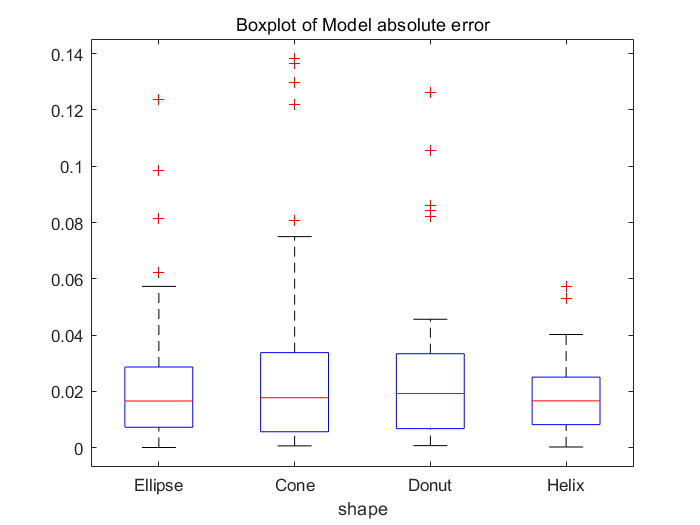
\includegraphics[width=2.5in]{Model.png}
\caption{Graphic model of artificial neural network (hidden layers).}
\label{fig_ANN}
\end{figure}
In our case, we adopt the regression function of ANN. Specifically, we use the Multi-layer Perceptron regressor. This regressor fits the training data iteratively. The loss function is defined as the Mean Square Error (MSE) between the predicted value and the real value. At each time step the partial derivatives of the loss function with respect to the model parameters are computed to update the parameters.

Practically, we use the off-the-shelf $MLPRegressor$ from scikit-learn library of Python. Experiment results show that this function is sufficient for our purpose.

\section{System Design}
Given Eq.\ref{ellipsoid_formula} above, we made an assumption that the map from relevant factors $K_p, K_m, f$ etc. to the effective thermal conductivity of the composite material is a non-linear relationship. While this relationship varies among different particle shapes, it can be generally captured by ANN as the weight parameters in the neurons. We assume that by generating data from a known particle shape, we can train the neural network to fit the data. As a result, the ANN model trained from a particular particle shape data can be used to replace the analytical formula that generate the data. The actual result is evaluated in the section below.

\subsection{Generalized Shape Factor}
On basis above, we want to extend the function of this ANN model by generalizing it to fit for other particle shapes. As in the misoriented ellipsoidal particle case shown in section \ref{sectionEMT}, the shape of the ellipsoidal particle is characterized by its aspect ratio. By generalizing this definition, we expect to assign each particle shape with a particular number to characterize its shape, referred to as generalized shape factor (GSF). This GSF can be plugged into the analytical formula or the ANN model to predict the thermal conductivity. 

To solve this generalization problem, we used another ANN model, with conventionally adopted parameters for particle shapes: volume, surface area and projection areas, as input and estimate the GSF as output.

\subsection{Data generation}
To obtain the training data, we use the Eq.\ref{ellipsoid_formula} above. Specifically, we randomly generate values for $K_p, K_m, f$ and length of two axes of the ellipsoid $a_1, a_3$ (assume $a_2 = a_1$), then plug in Eq.\ref{eq_Lii} to compute $L_{ii}$. The $L_{ii}$ is plugged into Eq.\ref{eq_beta} to obtain $\beta_{ii}$. Finally, $K_m, f, \beta_{ii}$ and $L_{ii}$ are plugged in Eq.\ref{ellipsoid_formula} to compute $K^*$, the thermal conductivity of the composite material. For simplicity, we narrow the range of parameters as below.
\begin{itemize}
\item $K_p$, $K_m \in (0, 20]$;
\item $f \in (0,1]$;
\item $a_1, a_3 \in \lbrace0.1, 0.2, ..., 0.9, 1.0\rbrace$
\end{itemize}

With the above restriction, we generate 100,000 entries of data as our training set. For each entry, the target conductivity value $K^*$, volume of the particle $V$, surface area of the particle $S$ and Projection areas from three directions $Pro_i \; (i = 1,2,3)$ are computed and recorded.
\subsection{K model}
K model is the ANN model trained to predict the thermal conductivity of the composite material. The input values are $K_p, K_m, f$ and $p$, and the output is the effective thermal conductivity $K^*$.
\subsection{P model}
P model is the ANN model trained to predict the GSF of the particular particle shape. The input values are $V, S$ and $Pro_{i}$, and the output value is the predictive GSF for this particular shape.

The result of the P model can be plugged into Eq.\ref{eq_beta} \ref{eq_Lii} and \ref{ellipsoid_formula} for evaluating the analytical thermal conductivity. Or, it can be plugged into the K model to give a predictive value of the thermal conductivity. We will evaluate the result of each method in the follow sections.
\section{Evaluation}
To-do BY Yu yi
\section{Limitation and discussion}
To-do By Yu yi

\section{Conclusion}
In this work, we present a system that is capable of quickly estimating the thermal conductivity of composite materials. As discussed above, it is feasible and reliable to use machine learning to predict the thermal conductivity of composite materials.The thermal conductivity predicted by our training model is very close to the real thermal conductivity, and is not limited to the prediction of elliptical particles. When we used the training model to predict other composite particle types, the prediction still provide results with acceptable error. Our research work can still be further improved in the future to estimate the thermal conductivity of various new composite materials. When this problem is solved, the prediction model can also be extended to predict other similar property problems, such as electrical conductivity.


% trigger a \newpage just before the given reference
% number - used to balance the columns on the last page
% adjust value as needed - may need to be readjusted if
% the document is modified later
%\IEEEtriggeratref{8}
% The "triggered" command can be changed if desired:
%\IEEEtriggercmd{\enlargethispage{-5in}}

% references section

% can use a bibliography generated by BibTeX as a .bbl file
% BibTeX documentation can be easily obtained at:
% http://mirror.ctan.org/biblio/bibtex/contrib/doc/
% The IEEEtran BibTeX style support page is at:
% http://www.michaelshell.org/tex/ieeetran/bibtex/
%\bibliographystyle{IEEEtran}
% argument is your BibTeX string definitions and bibliography database(s)
%\bibliography{IEEEabrv,../bib/paper}
%
% <OR> manually copy in the resultant .bbl file
% set second argument of \begin to the number of references
% (used to reserve space for the reference number labels box)
\begin{thebibliography}{1}

\bibitem{IEEEhowto:kopka}
H.~Kopka and P.~W. Daly, \emph{A Guide to \LaTeX}, 3rd~ed.\hskip 1em plus
  0.5em minus 0.4em\relax Harlow, England: Addison-Wesley, 1999.

\end{thebibliography}




% that's all folks
\end{document}